\documentclass[%
thesis=student,% bachlor's or master's thesis
coverpage=false,% do not print an extra cover page
titlepage=false,% do not print an extra title page
headmarks=true, % headmarks can be switched on or off
english,% or `german`
font=libertine, % use `libertine` font; alternatives: `helvet` / `palatino` / `times`
math=newpxtx, % math font `newpxtx`; alternatives: `ams`, `pxtx`
BCOR=5mm,% binding correction - adapt accordingly
coverBCOR=11mm% binding correction for the cover - adapt accordingly
]{tumbook}

\makeatletter %redefine some labels from the TUM template
\provideName{\@tum@examiner@}{Supervisor}{Themensteller} % or `Themenstellerin`
\provideName{\@tum@supervisor@}{Advisors}{Betreuer} % or `Advisor` / `Betreuerin`
\makeatother

\usepackage{booktabs}% for more beautiful tables
\usepackage{cleveref}% intelligent references

\usepackage{diffcoeff}
\usepackage{amsmath}
\newtheorem{definition}{Definition}[section]
\newtheorem{theorem}[definition]{Satz}

%Literatur
\usepackage[%
    backend=bibtex, %, or `biber` on more up-to-date systems
    sortcites, % sort automatically
    sorting=nty, % sort order
    safeinputenc, % solves problems with unicode-formatted author names etc.
    citestyle=alphabetic, %
    bibstyle=alphabetic, %
    hyperref=true, % provide clickable links
    maxbibnames=3, % shorten author list for more than 3 names
    maxcitenames=3, % use at most 3 names for key
    url=false, % do not print URLs
    doi=false, % do not print DOIs
    giveninits=true,
    ]%
{biblatex}
\addbibresource{literature.bib}

% automatische Anführungszeichen
\usepackage[autostyle=true]{csquotes}


\title{Implicit Context Condensation for Local Software Engineering Agents}
%%%\subtitle{A Comprehensive Study on LLM Context Management}

\author{Kirill Gelvan}

\degree{Master of Science}% or `Bachlor of Science`
\dateSubmitted{31. November 2025}% preferably use some universally recognized date format


\examiner{Prof.\@ Dr.\@ Gjergji Kasneci}% `Themensteller`
\supervisor{Felix Steinbauer\\Igor Slinko}% `Betreuer`


\begin{document}

\frontmatter
\maketitle

\section*{Zusammenfassung}
Eine kurze Zusammenfassung der Arbeit auf Deutsch.


\section*{Abstract}
A brief abstract of this thesis in English.


\cleardoublepage{}

\tableofcontents


\mainmatter{}


To use the \LaTeX{} templates provided here you will need to add the directory \verb|tum-templates| as a local package directory to your \LaTeX{} distribution. An easy way to do this is by setting the environment variable \verb|TEXINPUTS| to \verb|.//:| on Linux/Mac systems (meaning: search the current directory and its subdirectories for packages first, then use the usual search path). On a Linux or Mac you can compile this document to a PDF file in a terminal through the following commands (the first command needs to be issued only once):
\begin{verbatim}
export TEXINPUTS=.//:
pdflatex -output-directory=. master
bibtex master
pdflatex -output-directory=. master
\end{verbatim}


% ========================================
% CHAPTER FILES
% ========================================
% Each chapter is now in its own file for better organization
% ========================================
% CHAPTER 1: INTRODUCTION (MOTIVATION)
% ========================================
\chapter{Introduction}


% ========================================
% SECTION 1.1: THE CONTEXT LENGTH CHALLENGE IN LARGE LANGUAGE MODELS (LLMS)
% ========================================
\section{The Context Length Challenge in Large Language Models (LLMs)}

The ability of Large Language Models (LLMs) to effectively process long sequences of input text is fundamentally constrained by their architecture.
Specifically, Transformer-based LLMs face inherent limitations due to the self-attention mechanism, which scales quadratically with the number of tokens.
Much previous research has attempted to tackle this long context issue through architectural innovations, but these efforts often struggle to overcome a notable decline in performance on long contexts despite reducing computation and memory complexity.
While alternative attention mechanisms can make scaling closer to linear, they typically cannot achieve true linear scaling without quality drops on longer sequences.

The long context limitation presents a significant practical challenge, particularly in complex automated scenarios involving agents with many interaction turns.
This restriction is worsened in software engineering (SWE) agent applications, where operational trajectories frequently involve tool calls that generate unnecessarily long outputs.
SWE agents must perform tasks such as examining files and directories, reading and modifying parts of files, and navigating complex codebases.
However, pretrained models literally cannot work with sequences longer than N (e.g., 32,000) tokens, which prevents them from efficiently processing the accumulated history generated by these tools.

Context compression offers a novel approach to addressing this issue, motivated by the observation that a text can be represented in different lengths in an LLM while conveying the same information.
For example, the same information might be represented in various formats and densities without necessarily affecting the accuracy of the model's subsequent response.

\begin{figure}[hbt]
  \centering
  
\includegraphics[width=0.8\textwidth]{graphs/example1.jpeg}
  \caption{Comparison between base agent and our agent approaches for handling large observations exceeding LLM context length. The base agent fails when processing 5000-token observations directly, while our agent successfully compresses the observation to 256 embeddings before LLM processing, enabling continued task execution.}
  \label{fig:example1}
\end{figure}

The core goal of context condensation is precisely to leverage this potential density to enable LLM agents to execute tasks involving long chains of reasoning (or Chain-of-Thought, CoT) and more steps by condensing the environment observations.
Achieving this condensation improves the model's capability to handle long contexts while offering tangible advantages in improved latency and reduced GPU memory cost during inference.



% ========================================
% SECTION 1.2: Implicit Context Condensation
% ========================================

\section{Implicit Context Condensation}

The core concept of context condensation, motivated by the observation that text can convey the same information across different lengths and densities, leads directly to the discussion and comparison betwwee Implicit and Explicit Context Condensation.
Implicit Context Condensation approach moves beyond explicit, token-based summarization techniques by utilizing the inherent density of the LLM's latent space. 

Instead of relying on the discrete space of tokens, Implicit Context Condensation focuses on synthesizing long sequences of input text into continuous representations (embeddings). 
This is possible because the latent space of embeddings is much denser than the discrete space of tokens. 
Our goal is to enable LLM agents to execute tasks requiring long chains of reasoning by successfully condensing these observations.
% ========================================
% CHAPTER 2: BACKGROUND (FUNDAMENTALS)
% ========================================
\chapter{Background}


% ========================================
% SECTION 2.1: TRANSFORMER ARCHITECTURE AND POSITIONAL BIAS
% ========================================
\section{Transformer Architecture and Positional Bias}

Overview of the Transformer architecture and the role of position encodings (PEs) in injecting positional awareness and local inductive biases.
Discussion that position ID proximity often correlates with higher attention scores, establishing the importance of position layout in compression.

% \begin{definition}[Definitheit]
%   Hier definieren wir definitive Definitheit.
% \end{definition}
% 
% \begin{theorem}[vom X]
%   War wohl nix. Es gilt aber
%   \begin{align*}
%     \sum_{i=1}^{n} f_i(x) = \int \hat{f}(x) \dl{x}
%   \end{align*}
% \end{theorem}


% ========================================
% SECTION 2.2: PARAMETER-EFFICIENT LLM ADAPTATION (LORA)
% ========================================
\section{Parameter-Efficient LLM Adaptation (LoRA)}

Explanation of Low-Rank Adaptation (LoRA) as the chosen technique for parameter-efficiently adapting the LLM encoder during training.


% ========================================
% SECTION 2.3: AGENTIC ENVIRONMENT AND TOOL USE
% ========================================
\section{Agentic Environment and Tool Use}

Description of the necessity for LLM agents to process sequential action-observation data (trajectories) when interacting with a computer or environment.
Introduction to the tools provided to the assistant agent, such as bash, submit, and str\_replace\_editor (a custom editing tool).

% ========================================
% CHAPTER 3: RELATED WORK (WHAT WAS PREVIOUSLY DONE)
% ========================================
\chapter{Related Work}

\textbf{note: here i write "what was previously done". see 3.4 for that}


% ========================================
% SECTION 3.1: ARCHITECTURAL APPROACHES FOR LONG CONTEXT MODELING
% ========================================
\section{Architectural Approaches for Long Context Modeling}

Long-context modeling must address the quadratic cost of vanilla self-attention \cite{vaswani_attention_2017} while preserving task-relevant dependencies over thousands of tokens.

A useful taxonomy distinguishes:
\begin{itemize}
    \item attention variants that alter the attention operator itself;
    \item explicit compression methods that reduce the input via retrieval or summarization;
    \item implicit compression methods that learn compact, decoder-friendly representations without exposing full inputs during inference.
\end{itemize}

We briefly review each group and summarize advantages and limitations.

\paragraph{Attention variants.}
Sparse and local/windowed patterns reduce pairwise interactions to achieve sub-quadratic cost.
Windowed attention restricts each token to a fixed neighborhood and optionally augments a small set of global tokens to propagate long-range information.
Longformer combines sliding windows with learnable global tokens for long documents \cite{beltagy_longformer_2020}.
Block- and mixed-sparsity patterns (e.g., banded + random) as in BigBird provide theoretical expressivity and empirical gains on long sequences \cite{zaheer_bigbird_2020}.
Sparse Transformers \cite{child_sparse_2019} introduced fixed sparse patterns for scalable generation.
Advantages include improved memory/computation and strong local modeling.
Disadvantages include potential failures to route cross-window interactions when global tokens or connectivity patterns are insufficient, and hardware inefficiencies for irregular sparsity.

Linear-time approximations further change the attention operator.
Kernelized attention (Transformers-as-RNNs) linearizes softmax attention for autoregressive decoding \cite{katharopoulos_transformers_2020}.
Linformer projects keys/values along sequence length to attain linear complexity \cite{wang_linformer_2020}.
These methods offer asymptotic gains and longer feasible contexts.
However, they can underperform full attention on tasks requiring precise long-range interactions or exact softmax geometry.
They also introduce approximation/projection hyperparameters that affect quality.

\paragraph{Explicit compression.}
Retrieval-augmented generation (RAG) or summarization-based pipelines reduce the effective input by selecting or rewriting content before decoding.
RAG retrieves top-$k$ passages from an external corpus and conditions generation on them.
This approach improves knowledge-intensive tasks while decoupling parametric and non-parametric knowledge \cite{lewis_rag_2020}.
Abstractive summarization pre-compresses long inputs into concise proxies (e.g., PEGASUS pretraining with gap-sentence objectives) \cite{zhang_pegasus_2020}.
Benefits include controllable compute and access to external knowledge.
Drawbacks include selection bias, retrieval latency, brittleness to retrieval errors, and potential loss of details critical for downstream reasoning.

\paragraph{Implicit compression.}
Here, the idea is to produce task-adapted representations (often embeddings) that a model uses during inference, rather than the input itself.
Examples include learned soft/prefix prompts for steering frozen decoders \cite{li_prefix_2021,lester_prompt_2021}.
Other examples include tokenized memories trained to preserve answer-relevant information.
Implicit methods maintain a tight interface to the model.
They can reduce latency and memory without external retrieval.
A key challenge of implicit compression is that, by condensing input into a compact intermediate representation, some information may inevitably be lost and cannot be recovered with perfect fidelity. 
This may limit the utility of compressed representations, especially when critical details are omitted during the compression process.

Taken together, attention variants trade exactness for structure or approximation.
Explicit compression trades completeness for selection.
\textbf{TODO: this is bullshit but make a change to section 4. we like implicit -> so we found ICAE---} --- Implicit compression trades human readability for decoder-optimized compact interfaces.

% Insbesondere weisen wir auf den wunderbaren Artikel von \textcite{Edmonds:1965} und auf~\cite{GareyJohnson:1979} für weitere Hintergründe.


% ========================================
% SECTION 3.2: SOFT PROMPTING, CONTEXT DISTILLATION, AND CONTINUOUS-THOUGHT REPRESENTATIONS
% ========================================
\section{Soft Prompting, Context Distillation, and Continuous-Thought Representations}

Soft prompting is a method for conditioning large language models by learning continuous prompt vectors or prefix tokens rather than discrete text. 
These learned vectors are typically prepended to the model's input sequence and serve as a compact, trainable interface for adapting frozen decoders.
Classic methods in this category include prefix-tuning \cite{li_prefix_2021} and prompt tuning \cite{lester_prompt_2021}.
Both approaches involve optimizing a small set of continuous embeddings that steer the model toward desired behavior without full-scale model finetuning.
This parameter-efficient interface enables flexible adaptation and can be tuned for domain- or task-specific goals.
Because the prompt vectors are not constrained to map onto human-readable tokens, they can condense much more information than would be possible with standard textual prompts.

In practical, agentic settings the challenge of long or growing histories becomes acute (???).
%Models can distill the relevant information into a compact embedding or set of memory tokens.
%This reduces latency and memory overhead, as only condensed facts are passed forward during multi-step interactions.
%Examples of this pattern include ReAct-style prompting, which accumulates observations and actions over iterative reasoning steps \cite{yao_react_2022}, and Toolformer, which learns to use tools with self-supervised trajectories and requires summarizing complex action histories \cite{schick_toolformer_2023}.
%A scientific motivation for context distillation and soft prompting is that the resulting compression can be optimized directly for downstream utility, such as task success, rather than mere faithfulness to the original text.
%By learning what to keep and what to discard, these methods can mitigate biases and error propagation that affect explicit retrieval or summarization.

\textbf{CoConut} (Chain of Continuous Thought) \cite{coconut_placeholder,arxiv_2412_06769} generalizes the concept of soft prompting by moving away from natural language tokens altogether and enabling reasoning directly in latent, continuous spaces.
Instead of relying on explicit tokenization and sequence rewriting, CoConut leverages the model's own hidden states as a "continuous thought" vector.
After processing an input, the final hidden state (or a structured set of latent embeddings) is fed back as a contextual scaffold for further reasoning steps.
% Unlike prompt tuning, which fixes a learned vector prepended to all inputs, CoConut operates on an ever-evolving latent summary, tailored to the agent’s state as the interaction progresses.
Experiments show that directly reasoning in the model's own latent space improves downstream performance for tasks with extended, multi-step dependencies, outperforming classic chain-of-thought prompting.
By discarding the constraints of discrete tokenization, CoConut demonstrates that agentic LLMs can reason, plan, and retain context in a fundamentally more expressive and compact way.


% ========================================
% SECTION 3.3: THE IN-CONTEXT AUTOENCODER (ICAE) FRAMEWORK
% ========================================
\section{The In-Context Autoencoder (ICAE) Framework}

\textbf{TODO: I am very lost on where and how to write about ICAE. 
I guess here should be none, but then I need smth to compare 3 ideas from 3.1?
Then I also need ICAE in 4 and 5 somehow. Also 4.2 needs it but 4.3 is the same (expl. of AE vs LM for 50/50)}

ICAE \cite{ge_-context_2024} is closely related to the above implicit compression paradigm.
An encoder (often a LoRA-adapted copy of the base LLM) reads a long context and emits a small set of learnable \emph{memory tokens}.
A frozen decoder (the base LLM) then conditions on these tokens plus the downstream prompt to generate outputs.


ICAE differs from heuristic summarization in that the representation is optimized for decoder consumption rather than human readability.
It also differs from sparse or windowed attention in that the decoder still operates with dense attention over a small set of memory tokens.
ICAE differs from explicit RAG in that no external retrieval is required at inference \cite{beltagy_longformer_2020,zaheer_bigbird_2020,lewis_rag_2020}.
Compared to purely recurrent memory, ICAE offers direct, content-dependent access via attention over a small set of tokens.
This avoids long chains through recurrent states.



\section{Some attempts to do the same thing?}

Tobias' blogpost from openhands is not implicit, but explicit. so i have no knowledge of the same solutions using implicit compression?

Should write here about the other solutions for our problem/dataset? but what are those?
% ========================================
% CHAPTER 4: METHODS (CONCEPTUAL: ARCHITECTURE, DATA, AND TRAINING PROCEDURES)
% ========================================
\chapter{Methods}

\textbf{note: here I write "what am i doing on top of other methods" I write it conceptually. if i need results maybe reference to the next chapter.}



% ========================================
% SECTION 4.1: CONCEPTUAL SETUP AND AGENTIC DATA ACQUISITION
% ========================================
\section{Data Acquisition and Setup}

\subsection{SWE-bench}
We have chosen to use the SWE-bench \cite{jimenez2024swebench} dataset for our experiments.
It is a well known dataset for evaluating the performance of SWE agents.
It contains a large number of SWE tasks, each with a set of instructions and a set of expected outputs.
They were collected from real life GitHub issues. 
We have chosen to work with a subset -- SWE-bench Verified \cite{swebench-verified}.
It is a subset of the SWE-bench dataset that contains only the tasks that have been verified to be correct.

\subsection{Tools and Interaction Protocol (setup?)}
We follow the SWE-smith setup for SWE-bench Verified \cite{jimenez2024swebench}, where the assistant agent interacts with the environment through a minimal toolset and a fixed protocol. 
Concretely, the available tools are a shell interface (\texttt{bash}), a submission tool (\texttt{submit}), and a custom editing utility (\texttt{str\_replace\_editor}).
These tools generate the observations that accumulate within the trajectory context.
The exact SWE-smith prompt (and the tools description) is provided in Appendix~\ref{app:swe-smith-prompt}.
It should be noted that this method does not use function calling functionality of the model. 
While some models support a special format for function calling (e.g. additional fields for the tools descriptions etc.), in this case we just use the tools as described in the prompt.

\paragraph{The \texttt{str\_replace\_editor}.}
This is a stateful file editor that supports viewing, creating, and editing files with precise, line-exact operations.
Its state persists across steps, enabling consistent multi-edit workflows. 
The interface exposes the following commands: \texttt{view}, \texttt{create}, \texttt{str\_replace}, \texttt{insert}, and \texttt{undo\_edit}. 

For deterministic edits, \texttt{str\_replace} requires \texttt{old\_str} to match exactly one or more consecutive lines in the target file, including whitespace.
The \texttt{new\_str} content replaces the matched block.
The \texttt{insert} command appends \texttt{new\_str} after a specified line number.

By this, there is a lot of tools combined into one, but it works well as described in \cite{swe-smith}, so we adopt it. 
And also to be comparable to other open sourced scores.

\subsection{Agentic Trajectories as Data}
We treat sequential action--observation interactions (trajectories) as training data.
These trajectories were obtained using a strong teacher model (e.g., Claude Sonnet 3.7) on the SWE-bench Verified dataset to produce high-quality inputs suitable for futher training.
The setup for generating these trajectories follows the SWE-smith setup closely\cite{swe-smith}.

% ========================================
% SECTION 4.2: ICAE MODEL ARCHITECTURE FOR AGENTIC APPLICATION
% ========================================
\section{ICAE Model in Agentic Setup}

\subsection{ICAE Components}
As described previously, the ICAE \cite{ge_context_2024} consists of two modules: a lightweight encoder (implemented via a LoRA-adapted LLM) and a fixed decoder (the LLM itself).
The encoder processes the long trajectory context and generates a fixed number of learnable memory token.

We use the encoder for every environment observation (\textbf{TODO: picture here?})
So, more in detail, the encoder is only applied if all of the next are true:
\begin{itemize}
  \item The text is an observation (i.e. response from the environment, not the action)
  \item The text is longer or equal than 256 tokens
\end{itemize}
The actions are short and do not require compression, while the observations can be long and complex.
Due to the nature of the ICAE framework, the compression produces a fixed number of memory tokens, which we fix at 256.
Applying the encoder to the shorter texts would be a waste of resources and would create a mismatch between the training and the validation settings.
You can see the example of this in figure \ref{fig:ser1} and \ref{fig:ser2} from Chapter~\ref{chap:5}.

The ICAE framework design turns a long, potentially unwieldy context into a compact representation that the decoder can efficiently consume, improving latency and memory footprint while preserving fidelity for downstream tasks. 
The number of memory tokens controls the compression ratio (e.g., $4\times$ or higher), and the position-ID placement of these tokens influences how readily the decoder can access stored information (cf. Section~2.1) \cite{ge_-context_2024}.

Beyond the high-level description, Figure~\ref{fig:icae} depicts the encoder–decoder split. 
On the left, the encoder ingests the full context (e.g., a text) and produces a fixed number of memory tokens. 
On the right, the frozen decoder receives these tokens and a tokens
During pretraining, the encoder is optimized so that the decoder can reconstruct the original text and continue language modeling (50/50 chance of being used).
During fine-tuning, the objective emphasizes answering prompts correctly given only the memory tokens and the task prompt.
In practice, the encoder is frequently adapted with parameter-efficient methods such as LoRA \cite{hu2021lora}, whereas the decoder remains frozen to preserve the capabilities of the base model.
\begin{figure}[hbt]
  \centering
  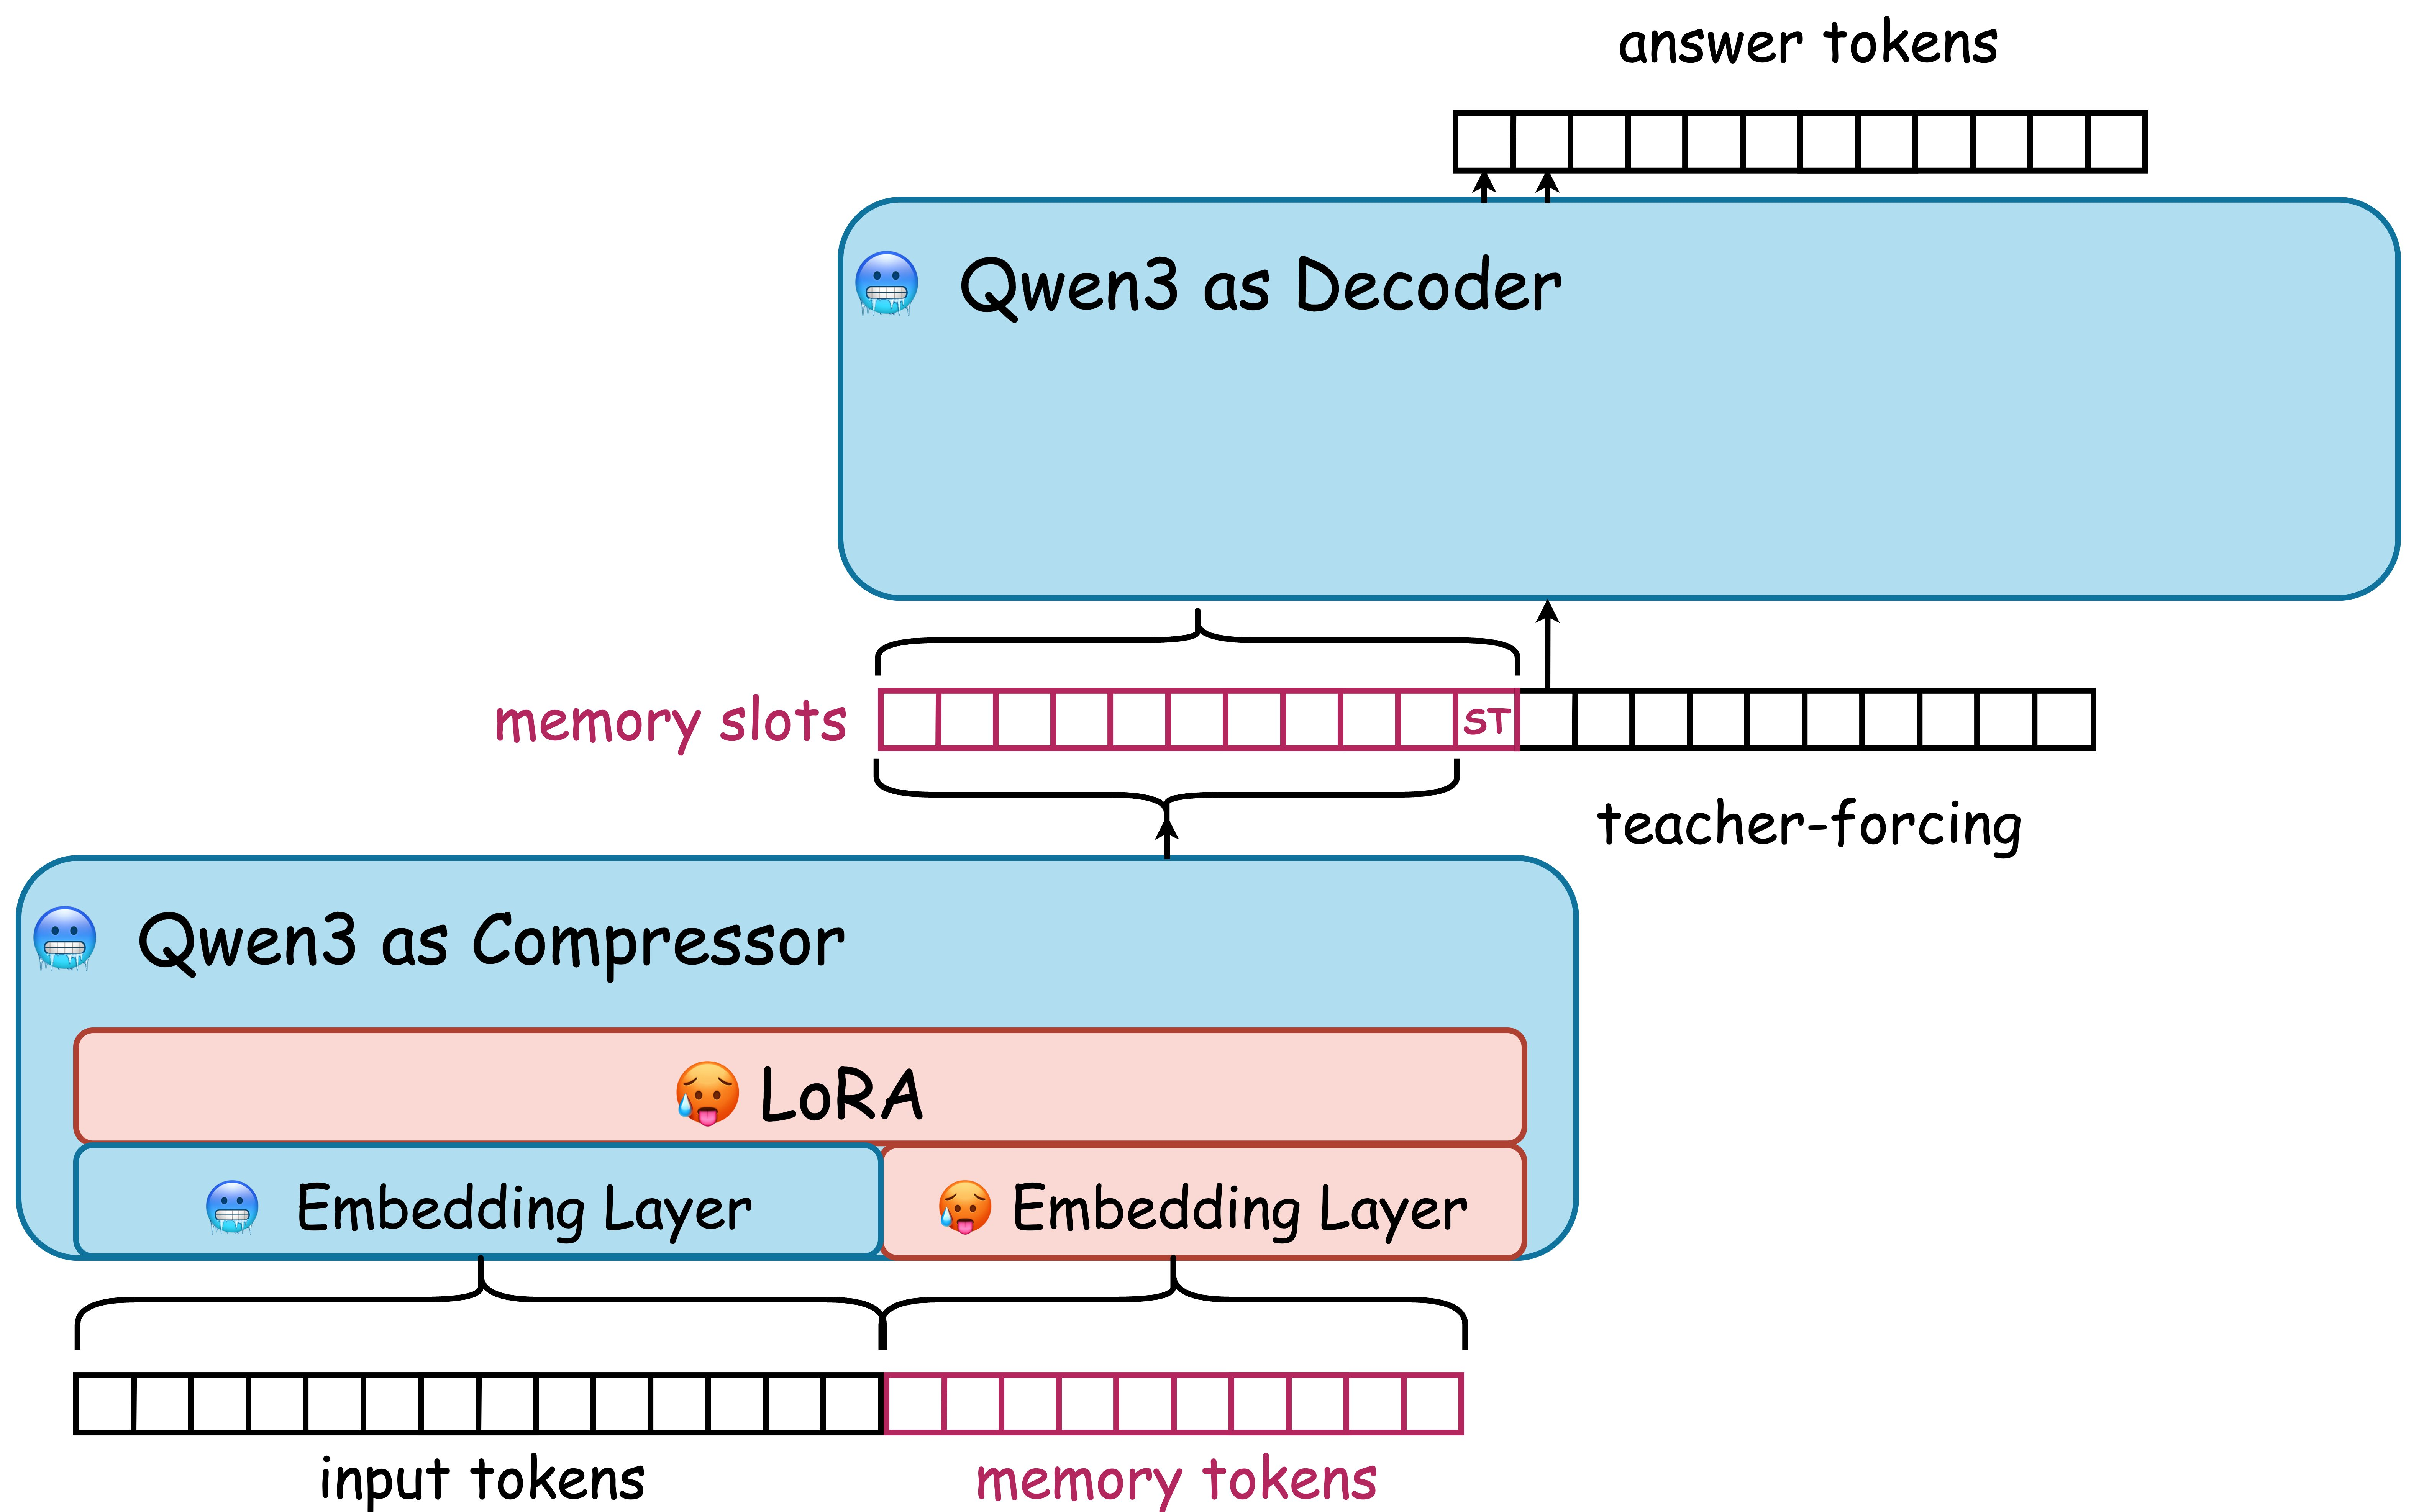
\includegraphics[width=0.8\textwidth]{graphs/icae.jpeg}
  \caption{In-Context Autoencoder (ICAE) framework architecture}
  \label{fig:icae}
\end{figure}

\subsection{Base Model Configuration (Qwen3)}
We use the Qwen3 model family (specificaly Qwen3-8B) as the base LLM. 
To make things simpler, we explicitly disable long-form "thinking" during decoding by inserting the token sequence \texttt{\textbackslash think \textbackslash think} with a newline marker (\texttt{\textbackslash n}) in between.
This is exactly how the authors of \cite{qwen3} recommend disabling thinking.
This prefix makes the model "believe" it has already produced intermediate thoughts (empty in this case), while in fact no additional content is generated.
We found that deleting or leaving this prefix in the history does have an inretesting affect the quality of the model, we describe this in more detail in Section~\ref{sec:5.6}.

It should also be noted that the authors of \cite{ge_context_2024} have only worked with older models (such as Llama2 and Mistral-v0.1), and only publish the weights of the latter.


% ========================================
% SECTION 4.4: TRAINING PROCEDURES BASED ON QWEN3
% ========================================
\section{Training Procedures and Evaluation}

\subsection{Pretraining (PT)}
Our pretraining procedure follows the original ICAE formulation~\cite{ge_-context_2024}.
We use two primary self-supervised objectives:
\begin{enumerate}[label=(\roman*)]
    \item \textbf{Autoencoding (AE)}, where ICAE restores the original input text from its memory slots (prompted by a special token \texttt{[AE]}).
    \item \textbf{Language Modeling (LM)}, which predicts the continuation of the context (prompted without any special tokens) to improve generalization and prevent overfitting to the AE task.
\end{enumerate}
This pretraining was performed on the dataset SlimPajama-6B \cite{pajama6b}\footnote{\url{https://huggingface.co/datasets/DKYoon/SlimPajama-6B}}.
It is a common text dataset, that is used for pretraining LLMs, consisting of 6 billion tokens (a random 1\% of the original 627B tokens).
The dataset that authors used in their original paper "The Pile" was unavailable.

It should be noted that only LoRA weights of the encoder are trained here (specifically only form Q and K matrices of the attention layers).
So, in theory, we are training the encoder to encode the context into such embeddings, that the decoder will be able to reconstruct the original context from them or to continue the text from the context.

\begin{figure}[hbt]
  \centering
  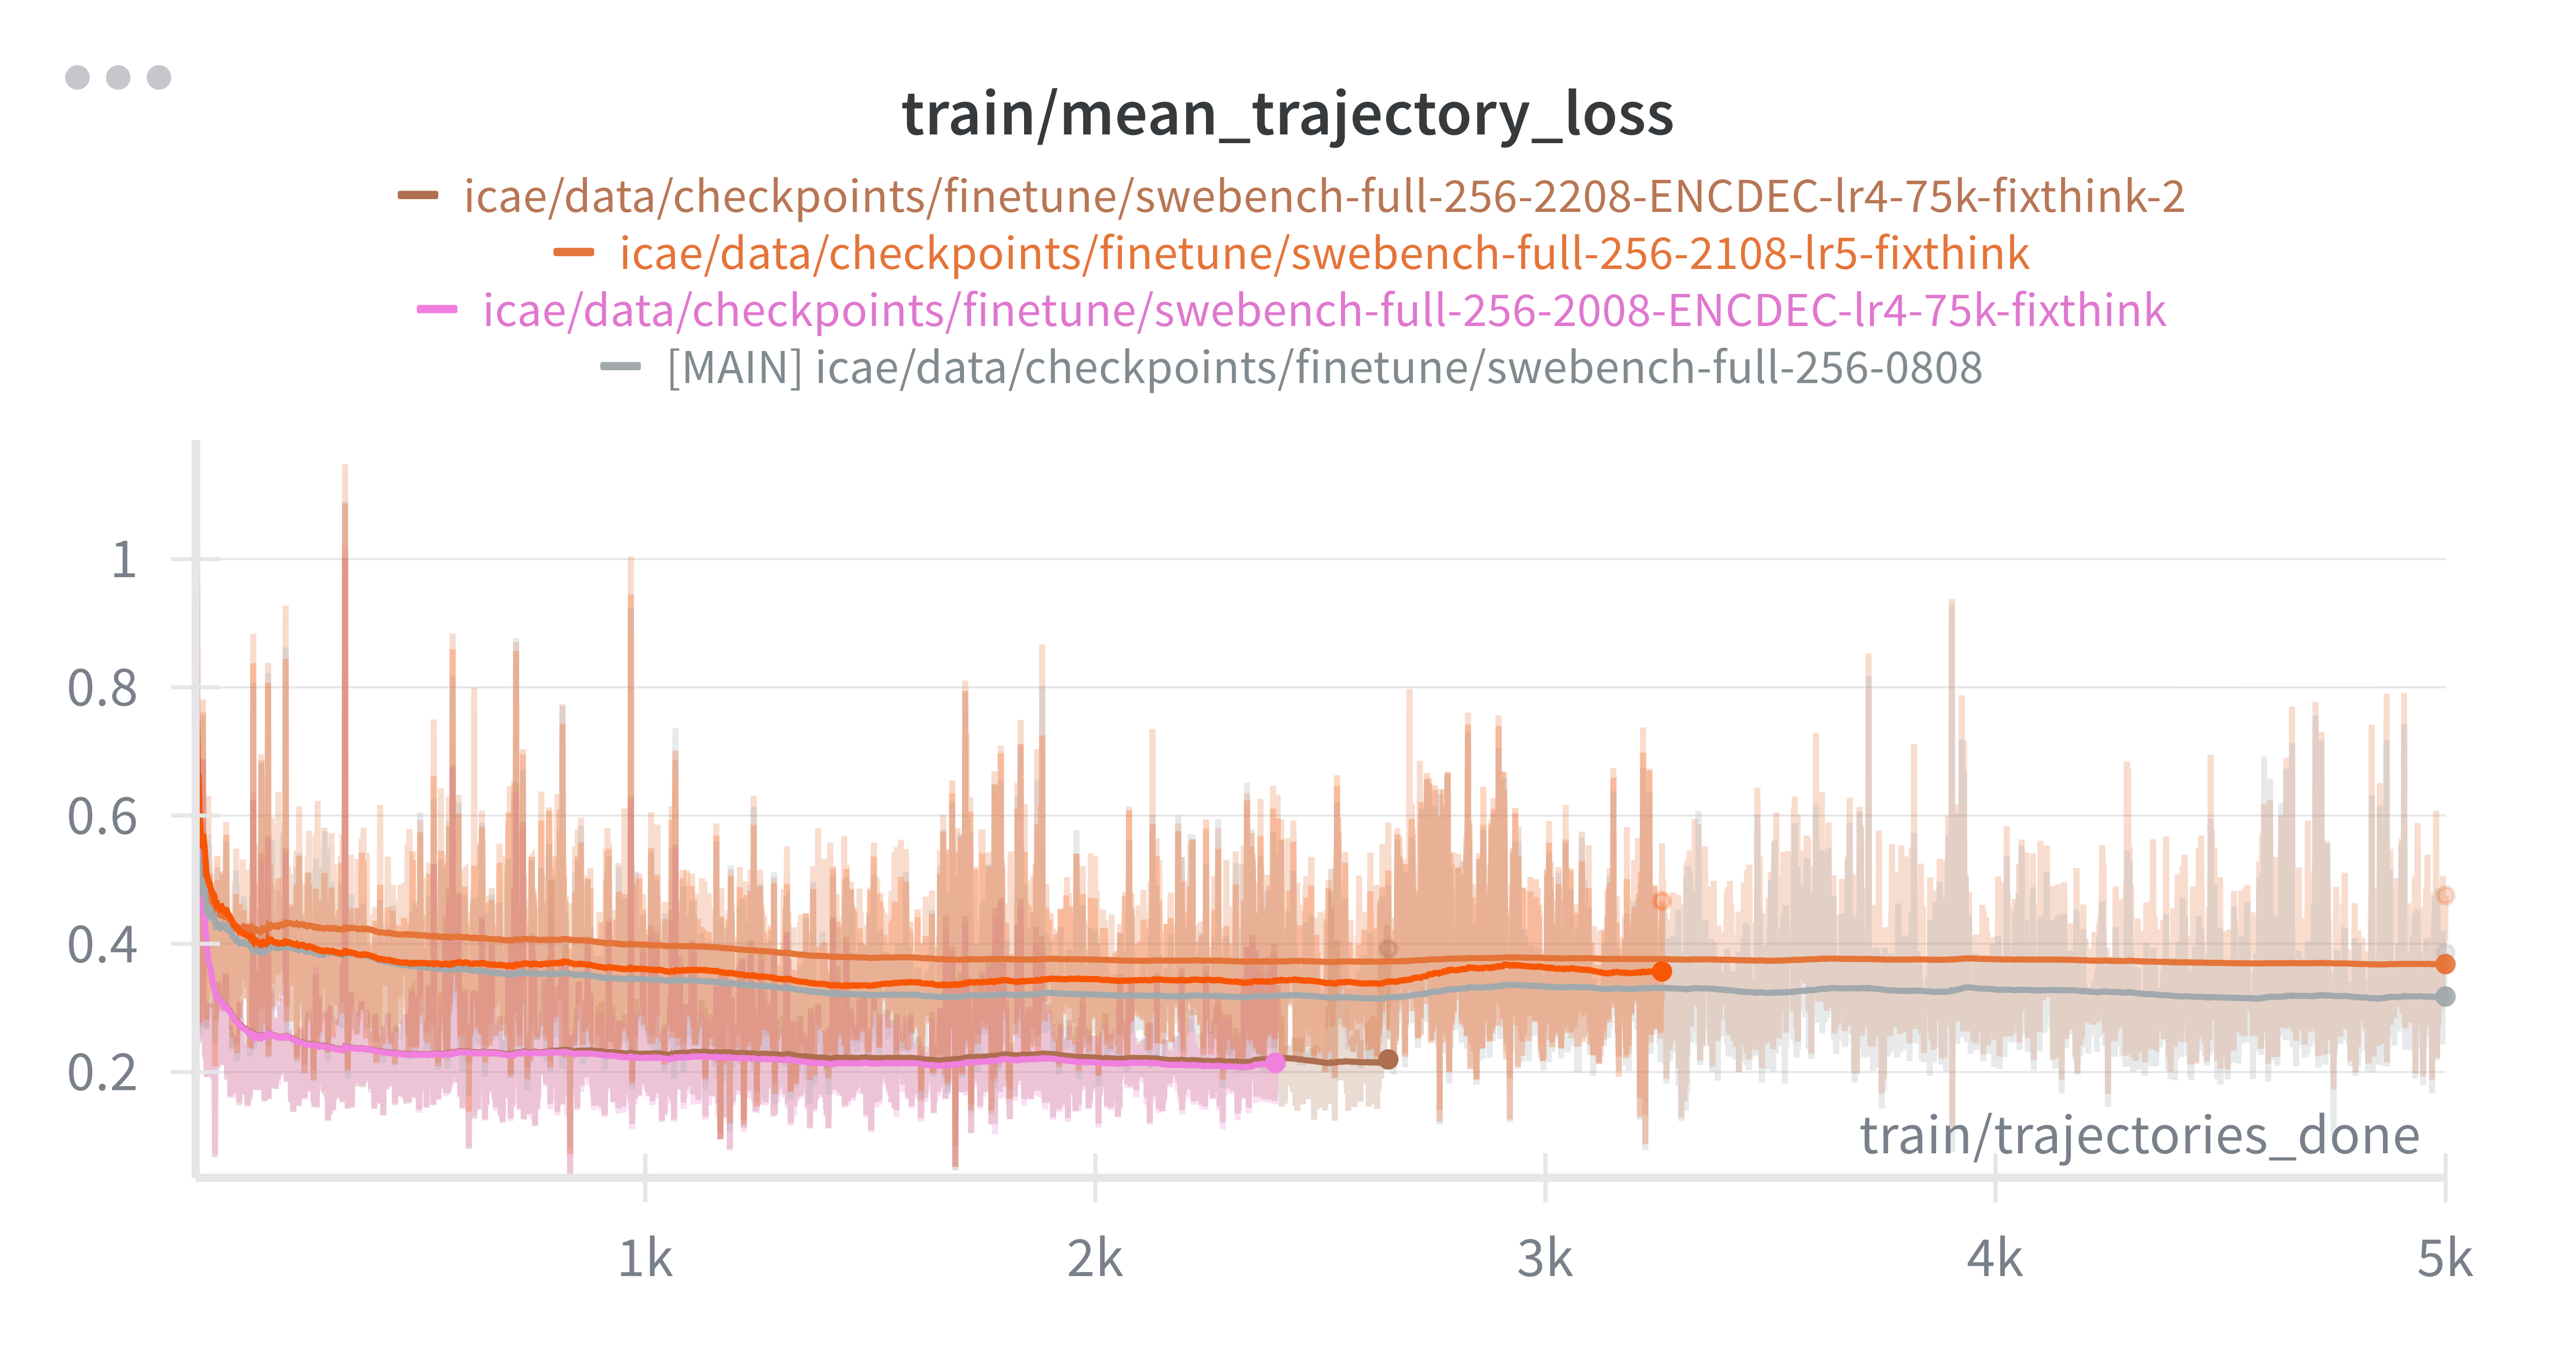
\includegraphics[width=0.9\textwidth]{graphs/pt_losses.png}
  \caption{Pretraining loss curves averaged by trajectory}
  \label{fig:pt_losses}
\end{figure}

\subsection{Fine-Tuning (FT)}
After pretraining, ICAE is fine-tuned using trajectories from SWE-bench Verified (the proccess of obtaining trajectories is described in Section~4.1.3).
Here as well only the LoRA weights are trained.
The fine-tuning objective maximizes the probability of generating the correct agent action (i.e. tool call) conditioned on the memory slots (if the encoder is applied at the current step) and the previous history (???)

It should be noted that the training is only applied to the encoder part, while the decoder is frozen.


During training, the backpropagation process constrains us to optimize over single-step transitions:
So at timestep \(k\), the encoder compresses the observation \(o_{k-1}\) into embeddings. Then, the decoder generates the action \(a_k\) given the memory slots and the previous history.
Then, token-by-token of \(a_k\) we backpropagate the loss through the decoder and the encoder, making an update of the LoRA weights of the encoder.
Crucially, whenever an observation exceeds 256 tokens, the encoder compresses it into a fixed set of 256 memory tokens (continuous embeddings), and these memory tokens replace the original text in the accumulated history.
If the observation is longer than 1024 tokens, we apply the encoder multiple times, preserving the compression ratio, following the authors of \cite{ge_context_2024}.
Consequently, the model never processes the full raw text of long observations during subsequent steps—it only conditions on the compact memory representations.

For example, consider a trajectory:
\begin{enumerate}
  \item \textbf{System prompt} (text): initial instructions and tool descriptions.
  \item \textbf{Task description} (text): user-provided issue or goal.
  \item \textbf{Action 1} (text): e.g., \texttt{bash: ls -la}.
  \item \textbf{Observation 1} (short text, $<256$ tokens): directory listing, kept as-is.
  \item \textbf{Action 2} (text): e.g., \texttt{str\_replace\_editor: view file.py}.
  \item \textbf{Observation 2} (long text, $\geq 256$ tokens): entire file content, compressed into 256 memory tokens.
  \item \textbf{Action 3} (text): e.g., \texttt{str\_replace\_editor: str\_replace ...}.
  \item \textbf{Observation 3} (long text): edit confirmation with context, again compressed into memory tokens.
  \item \textbf{Action 4} (text): e.g., \texttt{bash: pytest}.
  \item \textbf{Observation 4} (short text): test results summary, kept as text.
  \item \textbf{Action 5} (text): \texttt{submit}.
  \item \textbf{End}.
\end{enumerate}
So, in this example, the encoder is applied 2 times (steps 7 and 9), while the decoder is applied 5 times (steps 3, 5, 7, 9, 11).

At training time, each step's loss is computed independently: the model learns to predict \(a_k\) from the prefix ending at \(o_{k-1}\), where any long observation has already been replaced by its memory tokens.
At inference time, the same replacement occurs dynamically, ensuring consistency between training and deployment.
This design allows the model to handle arbitrarily long trajectories without exceeding context limits, as the effective history remains compact.

On figure \ref{fig:ft_losses} you can notice the sudden drop of the loss.
This is phenomenon found in \cite{PI}.
It appears due to the modification of positional encodings for the memory tokens.
We see the effect being the same as described by the authors.
In our experiments, it only appers if we apply the positional encodings manipulations.

\begin{figure}[hbt]
  \centering
  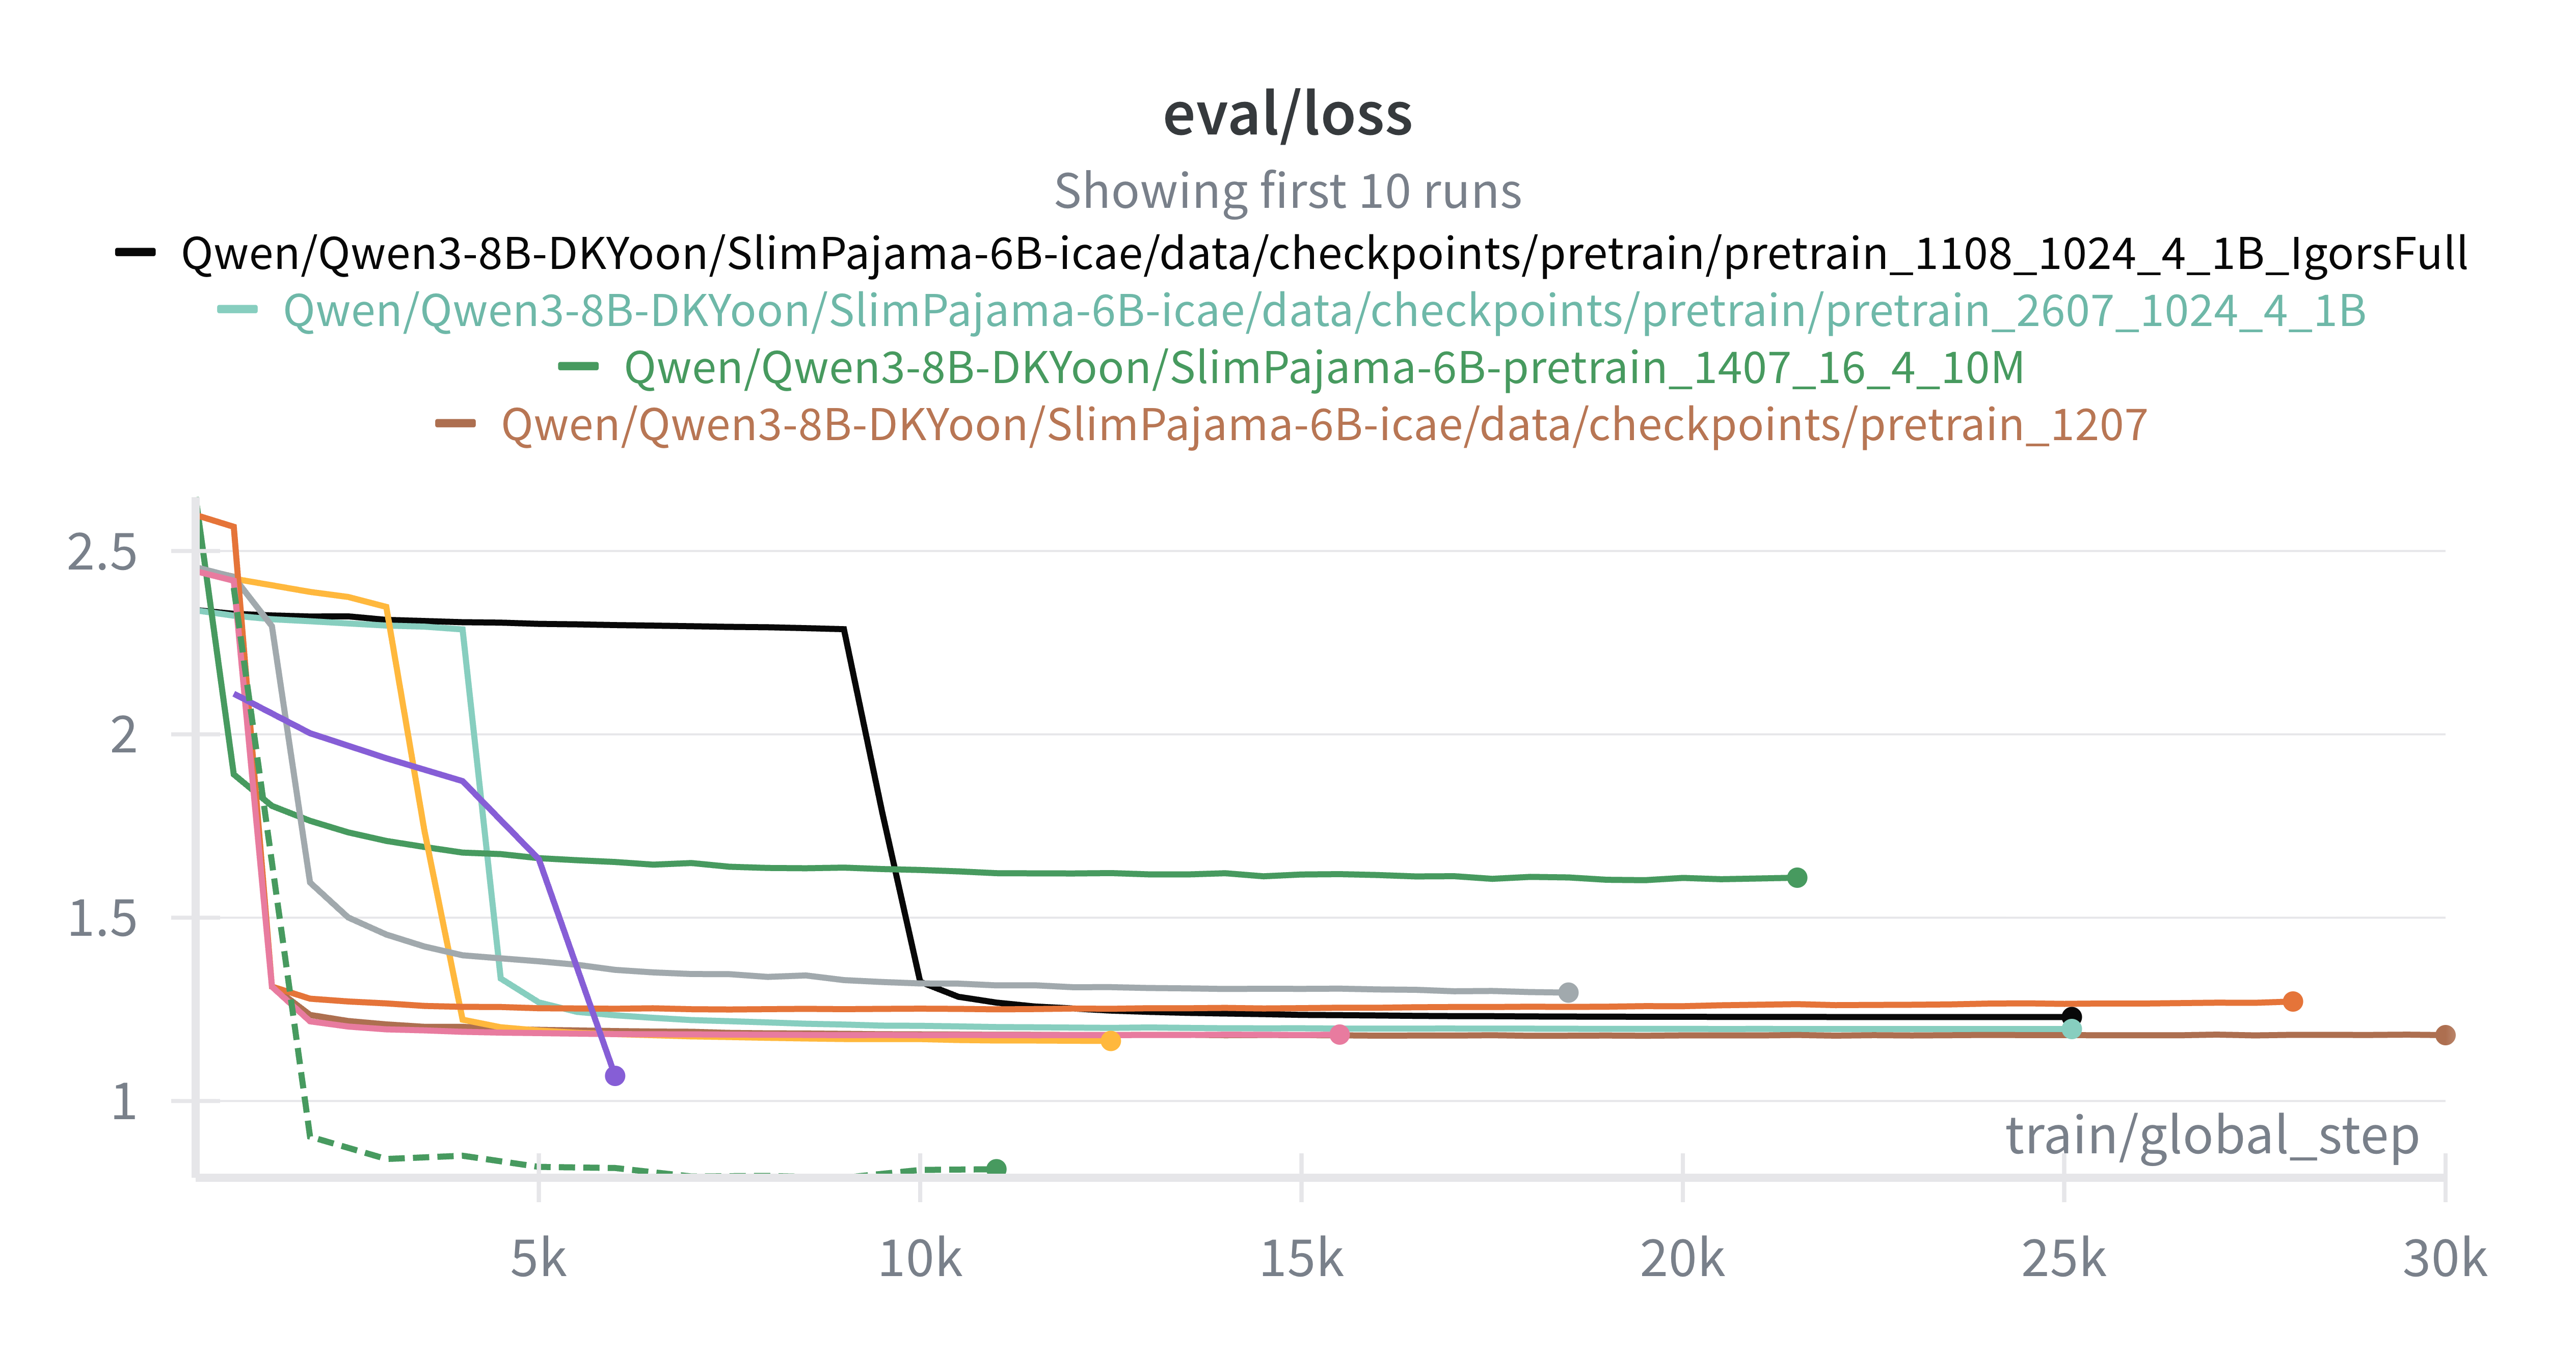
\includegraphics[width=0.9\textwidth]{graphs/ft_losses.png}
  \caption{Fine-tuning loss curves}
  \label{fig:ft_losses}
\end{figure}


\section{Code Reproduction and Testing Methodology}

\subsection{Key Metrics}
We report several metrics to evaluate our approach.
As a simple proxy metric, we measure token-wise accuracy —- averaged fraction of the guessed tokens that match the reference trajectory (note: this is measured with teacher forcing).
However, the most important metric is the number of successfully resolved issues on SWE-bench Verified, which directly reflects the model's ability to complete real-world software engineering tasks.
We also measure mean tool-call generation time to assess computational performance.

We note that measuring trajectory length is not particularly meaningful in our setting, as 8B-scale models frequently enter loops where they repeatedly call the same tool, artificially inflating trajectory length without making meaningful progress toward task completion.

% I believe this is not needed? at lease for now
%\subsection{Evaluation}
%In deployment, the accumulated history (trajectory) is first passed to the encoder, which condenses it into memory slots. The decoder (Qwen3) then uses these memory slots, conditioned by the current task prompt, to generate the subsequent action or response. The outcome is that the model operates with a much shorter effective context, improving latency and reducing GPU memory costs during inference.
%The final model is evaluated by deploying it to generate responses iteratively within the ICAE framework on the verified 500 subset of the SWE-bench Verified dataset.

\subsection{Code Reproducibility}
We reimplemented the ICAE framework from scratch, as the original authors' code was outdated and difficult to adapt to our experimental needs.
Our implementation is more modular and provides separate training pipelines for both pretraining (PT) and fine-tuning (FT).
We support pretraining on general text datasets (such as SlimPajama) and fine-tuning on both question-answering tasks (SQuAD) and agentic trajectories (SWE-bench).
We provide a link to our code repository\footnote{\url{https://github.com/JetBrains-Research/icae}} for transparency and reproducibility.



% ========================================
% CHAPTER 5: EXPERIMENTS AND EVALUATION (ACTUAL SETUPS AND RESULTS)
% ========================================
\chapter{Experiments and Evaluation}


% ========================================
% SECTION 5.1: INITIAL PROTOTYPE EXPERIMENTS: THE NECESSITY OF TRAINING
% ========================================
\section{Initial Prototype Experiments: The Necessity of Training}

The initial approach tested replacing hard tokens with soft/averaged continuous embeddings without fine-tuning. These prototype experiments, using methods like KV-cache hacks or direct embedding inputs in vLLM, demonstrated that scores decreased by more than 50\% on QA tasks (e.g., SQuAD context embed F1 dropped from 0.71 to 0.17 or 0.11). This negative result confirmed the hypothesis that training is necessary to effectively condense context into the latent space.


% ========================================
% SECTION 5.2: EVALUATION ON GENERAL TEXT RECONSTRUCTION
% ========================================
\section{Evaluation on General Text Reconstruction}

Pretrained ICAE demonstrated the ability to decompress general texts almost perfectly. High BLEU scores were achieved on datasets like PWC (99.1 for Mistral-7B, 99.5 for Llama-2-7B) and SQuAD (98.1 for Qwen3-8B), indicating that memory slots retained almost all context information for contexts up to 400 tokens. Analysis of reconstruction errors showed patterns similar to human memorization mistakes (e.g., restoring "large pretrained language model" as "large pretrained model"), suggesting the model selectively emphasizes or neglects information based on its understanding.


% ========================================
% SECTION 5.3: EVALUATION ON QUESTION ANSWERING TASKS (OFFLINE)
% ========================================
\section{Evaluation on Question Answering Tasks (Offline)}

When fine-tuned on QA tasks (SQuAD), ICAE-FT achieved high F1 (73) and Exact Match (69\%) scores, performing well compared to LoRA-FT baselines. The quality of the compressed representation was shown to significantly outperform summaries generated by GPT-4 under the same length constraint (128 tokens).


% ========================================
% SECTION 5.4: EVALUATION ON AGENTIC PERFORMANCE (SWE-BENCH)
% ========================================
\section{Evaluation on Agentic Performance (SWE-bench)}

Efficiency Results: ICAE compression led to measurable efficiency improvements, achieving a theoretically 10\% faster mean tool-call generation time than the vanilla baseline (e.g., 0.4880s vs 0.5437s). Furthermore, latency tests showed speedups of 2.2× to 3.6× in total time for inference. Token-wise Accuracy vs. Resolved Rate: Although token-wise accuracy performed on par with (or slightly better than) the vanilla Qwen baseline (e.g., 0.9089 vs 0.9000), this metric was noted to be problematic ("token-wise accuracy is bullshit") and decoupled from true task success. End-to-End Task Success: The primary negative finding was that the model with compression resolved significantly fewer than 50\% as many issues as the original Qwen model on the SWE-bench Verified dataset.


% ========================================
% SECTION 5.5: DISCUSSION OF AGENTIC FAILURE HYPOTHESES
% ========================================
\section{Discussion of Agentic Failure Hypotheses}

Hypotheses for the end-to-end performance degradation include Representation–behavior mismatch, where the compression perturbs the decoder's behavior necessary for tool use. Other factors include reconstruction quality falloff for specialized content like code files, and potential overfitting to labels demonstrated by high local accuracy but low resolved rates.

% ========================================
% CHAPTER 6: LIMITATIONS AND FUTURE WORK (WHAT CAN WE NOT COVER)
% ========================================
\chapter{Limitations and Future Work}


% ========================================
% SECTION 6.1: LIMITATIONS OF FIXED-LENGTH COMPRESSION
% ========================================
\section{Limitations of Fixed-Length Compression}

The methodology assumes that "all tokens in the context are equally important," aligning intrinsically with lossless compression (autoencoding), which becomes problematic under high compression ratios (lossy compression). The non-robustness of the approach is constrained by the hardcoded number of memory tokens (e.g., 256 tokens in discussion), defining the limitation of the approach as fixed-length feature extraction. Experimental results confirm that improvement attenuates or fails at high compression ratios (e.g., beyond 15x or 31x).


% ========================================
% SECTION 6.2: CONSTRAINTS ON MODEL SCALE
% ========================================
\section{Constraints on Model Scale}

Due to computational limitations, experiments were mainly conducted on Llama models up to 13 billion parameters.


% ========================================
% SECTION 6.3: OUTLOOK FOR FUTURE RESEARCH
% ========================================
\section{Outlook for Future Research}

Future work should explore validating the ICAE effectiveness on larger and stronger LLMs, as performance is expected to benefit more from more powerful target models. Potential extension to multimodal LLMs (images, video, audio) is suggested, as these modalities have greater compression potential.

% ========================================
% CHAPTER 7: CONCLUSION
% ========================================
\chapter{Conclusion}

\textbf{note: here I write "very high level overview of the whole thesis"}

% ========================================
% SECTION 7.1: SUMMARY OF ACHIEVEMENTS
% ========================================
\section{Summary of Achievements}

The ICAE \cite{ge_-context_2024} framework successfully achieves context condensation/feature extraction for general text, demonstrating high reconstruction quality (BLEU $\approx 99\%$) and measurable efficiency gains (speedup 2× to 3.6×).
The work provided insights into LLM memorization patterns, suggesting similarities to human memory encoding.


% ========================================
% SECTION 7.2: SYNTHESIS OF FINDINGS
% ========================================
\section{Synthesis of Findings}

Despite achieving efficiency and local accuracy on agent trajectories, the performance degradation in end-to-end task completion (resolved issues) highlights the critical gap between local context compression quality and robust decision-making in complex agentic settings.


% ========================================
% SECTION 7.3: POSITIONING THE WORK
% ========================================
\section{Positioning the Work}

The findings position this work within the broader research efforts on LLM context management, emphasizing the experimental results concerning condensation effectiveness across different data types, and suggesting caution when applying general compression methods to fine-grained, critical agent behaviors (code and tool use).

% ========================================
% APPENDIX SECTION
% ========================================
\appendix
\chapter{Appendix}


% ========================================
% APPENDIX SECTION A.1: TRAINING DETAILS AND HYPERPARAMETERS
% ========================================
\section{Training Details and Hyperparameters}
\label{app:training_details}

\subsection{Pretraining Configuration}

\begin{table}[h]
    \centering
    \small
    \begin{tabular}{ll}
        \toprule
        \textbf{Parameter} & \textbf{Value} \\
        \midrule
        Base Model & Qwen3-8B \\
        Dataset & SlimPajama-6B \\
        Learning Rate & $1 \times 10^{-4}$ \\
        Batch Size & 1 (with 8-step gradient accumulation) \\
        Training Steps & 100,000 \\
        Epochs & 3 \\
        Memory Size & 128 tokens (4× compression) \\
        LoRA Rank & 128 \\
        LoRA Target Modules & q\_proj, v\_proj \\
        Optimizer & AdamW \\
        Weight Decay & 0 \\
        Warmup Steps & 300 \\
        Max Gradient Norm & 2 \\
        Hardware & 1× NVIDIA H200 GPU \\
        Training Time & ~1 day 15 hours \\
        \bottomrule
    \end{tabular}
    \caption{Pretraining hyperparameters and configuration}
    \label{tab:pretrain_config}
\end{table}

\subsection{Fine-tuning Configuration}

\begin{table}[h]
    \centering
    \small
    \begin{tabular}{ll}
        \toprule
        \textbf{Parameter} & \textbf{Value} \\
        \midrule
        Base Model & Qwen3-8B \\
        Dataset & SWE-bench trajectories \\
        Learning Rate & $5 \times 10^{-5}$ \\
        Batch Size & 1 (with 1-step gradient accumulation) \\
        Training Steps & 150,000 \\
        Epochs & 5 \\
        Memory Size & 256 tokens \\
        LoRA Rank & 128 \\
        LoRA Target Modules & q\_proj, v\_proj \\
        Optimizer & AdamW \\
        Weight Decay & 0 \\
        Warmup Steps & 250 \\
        Max Gradient Norm & 2 \\
        Hardware & 1× NVIDIA H200 GPU \\
        Training Time & ~3 days \\
        Thinking Mechanism & Disabled \\
        \bottomrule
    \end{tabular}
    \caption{Fine-tuning hyperparameters and configuration}
    \label{tab:finetune_config}
\end{table}

\subsection{Reproducibility Resources}

To ensure full reproducibility, we publish our complete implementation including:
\begin{itemize}
    \item Complete ICAE framework for both pretraining and fine-tuning phases
    \item All training configurations and hyperparameters
    \item Full Weights \& Biases experiment logs for pretraining: \url{https://wandb.ai/kirili4ik/icae-pretraining}
    \item Full Weights \& Biases experiment logs for fine-tuning: \url{https://wandb.ai/kirili4ik/icae-swebench-finetune}
    \item Pretrained model checkpoints achieving 95\% reconstruction BLEU
    \item Fine-tuned models that outperform uncompressed baselines on SQuAD
\end{itemize}


% ========================================
% APPENDIX SECTION A.2: PROFILING SETUP AND LATENCY MEASUREMENT
% ========================================
\section{Profiling Setup and Latency Measurement}

Technical details of the test machine and runtime configuration used for latency measurements.


% ========================================
% APPENDIX SECTION A.3: DATASET CONSTRUCTION DETAILS (PWC)
% ========================================
\section{Dataset Construction Details (PWC)}

Details on the creation of the PWC dataset using GPT-4 to generate (context, prompt, answer) triples, including the prompt used for generation.


% ========================================
% APPENDIX SECTION A.4: DETAILED EVALUATION TABLES
% ========================================
\section{Detailed Evaluation Tables}

Comprehensive tables of model performance, including token-wise accuracy, mean tool-call time, and resolved issues for various ICAE \cite{ge_-context_2024} variants (e.g., Qwen-LoRA-FT, ICAE (Qwen-LoRA-FT) Qwen).


% ========================================
% APPENDIX SECTION A.5: CODE AND REPRODUCIBILITY
% ========================================
\section{Code and Reproducibility}

Note on the necessity of hosting all code on GitHub to ensure reproducibility.


% ========================================
% BACKMATTER SECTION
% ========================================
% Lists of figures and tables (may be removed if not needed)
\backmatter{}
\listoffigures% may be removed
\listoftables% may be removed

% ========================================
% BIBLIOGRAPHY SECTION
% ========================================
% Add any additional citations that haven't been referenced in the text
\nocite{Alspach:2008,GaleShapley:1962} % further literature that has not been explicitly referenced in the text
\printbibliography{} % print bibliography

\end{document}

%%% Local Variables:
%%% mode: latex
%%% TeX-engine: default
%%% TeX-command-extra-options: "-shell-escape"
%%% ispell-local-dictionary: "american"
%%% eval: (setenv "TEXINPUTS" ".//:")
%%% TeX-master: t
%%% End:
